\subsection{Sales Revenue Per Month}
This visualization displays total sales revenue by month to analyze changes in overall sales performance over time. A slicer that allows users to control which categories to include was incorporated to allow revenue comparisons across different product categories.
\begin{lstlisting}[language=SQL]
SELECT Month, SUM(SalesRevenue) AS TotalRevenue
FROM Sales
GROUP BY Month
ORDER BY Month;
\end{lstlisting}

\textbf{Visualization:}
\begin{center}
    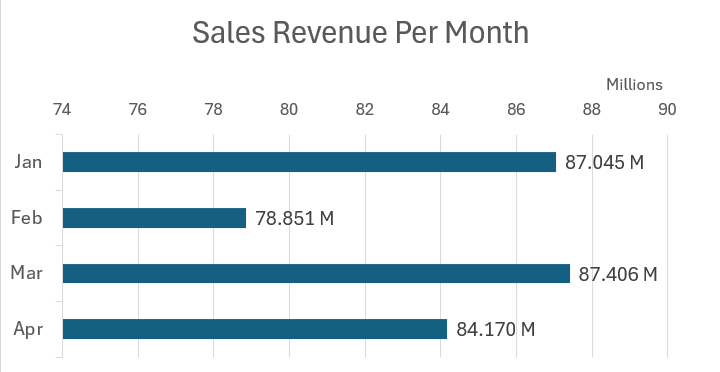
\includegraphics[width=1\linewidth]{Images/6.CHART_sales-revenue-per-month.png}
\end{center}
